%%%%%%%%%%%%%%%%%%%%%%%%%%%%%%%%%%%%%%%%%12pt: grandezza carattere
                                        %a4paper: formato a4
                                        %openright: apre i capitoli a destra
                                        %twoside: serve per fare un
                                        %   documento fronteretro
                                        %report: stile tesi (oppure book)
\documentclass[12pt,a4paper,openright,twoside]{report}
%
%%%%%%%%%%%%%%%%%%%%%%%%%%%%%%%%%%%%%%%%%libreria per scrivere in italiano
\usepackage[italian]{babel}
\usepackage{listings}
%
%%%%%%%%%%%%%%%%%%%%%%%%%%%%%%%%%%%%%%%%%libreria per accettare i caratteri
                                        %   digitati da tastiera come � �
                                        %   si pu� usare anche
                                        %   \usepackage[T1]{fontenc}
                                        %   per� con questa libreria
                                        %   il tempo di compilazione
                                        %   aumenta
\usepackage[latin1]{inputenc}
%
%%%%%%%%%%%%%%%%%%%%%%%%%%%%%%%%%%%%%%%%%libreria per impostare il documento
\usepackage{fancyhdr}
%
%%%%%%%%%%%%%%%%%%%%%%%%%%%%%%%%%%%%%%%%%libreria per avere l'indentazione
%%%%%%%%%%%%%%%%%%%%%%%%%%%%%%%%%%%%%%%%%   all'inizio dei capitoli, ...
\usepackage{indentfirst}
%
%%%%%%%%%libreria per mostrare le etichette
%\usepackage{showkeys}
%
%%%%%%%%%%%%%%%%%%%%%%%%%%%%%%%%%%%%%%%%%libreria per inserire grafici
\usepackage{graphicx}
%
%%%%%%%%%%%%%%%%%%%%%%%%%%%%%%%%%%%%%%%%%libreria per utilizzare font
                                        %   particolari ad esempio
                                        %   \textsc{}
\usepackage{newlfont}
%
%%%%%%%%%%%%%%%%%%%%%%%%%%%%%%%%%%%%%%%%%librerie matematiche
\usepackage{amssymb}
\usepackage{amsmath}
\usepackage{latexsym}
\usepackage{amsthm}
%
\oddsidemargin=30pt \evensidemargin=20pt%impostano i margini
\hyphenation{sil-la-ba-zio-ne pa-ren-te-si}%serve per la sillabazione: tra parentesi
					   %vanno inserite come nell'esempio le parole
%					   %che latex non riesce a tagliare nel modo giusto andando a capo.

%
%%%%%%%%%%%%%%%%%%%%%%%%%%%%%%%%%%%%%%%%%comandi per l'impostazione
                                        %   della pagina, vedi il manuale
                                        %   della libreria fancyhdr
                                        %   per ulteriori delucidazioni
\pagestyle{fancy}\addtolength{\headwidth}{20pt}
\renewcommand{\chaptermark}[1]{\markboth{\thechapter.\ #1}{}}
\renewcommand{\sectionmark}[1]{\markright{\thesection \ #1}{}}
\rhead[\fancyplain{}{\bfseries\leftmark}]{\fancyplain{}{\bfseries\thepage}}
\cfoot{}
%%%%%%%%%%%%%%%%%%%%%%%%%%%%%%%%%%%%%%%%%
\linespread{1.3}                        %comando per impostare l'interlinea
%%%%%%%%%%%%%%%%%%%%%%%%%%%%%%%%%%%%%%%%%definisce nuovi comandi
%
\begin{document}
\begin{titlepage}                       %crea un ambiente libero da vincoli
                                        %   di margini e grandezza caratteri:
                                        %   si pu\`o modificare quello che si
                                        %   vuole, tanto fuori da questo
                                        %   ambiente tutto viene ristabilito
%
\thispagestyle{empty}                   %elimina il numero della pagina
\topmargin=6.5cm                        %imposta il margina superiore a 6.5cm
\raggedleft                             %incolonna la scrittura a destra
\large                                  %aumenta la grandezza del carattere
                                        %   a 14pt
\em                                     %emfatizza (corsivo) il carattere
Alla mia famiglia, \\
che mi ha sempre sostenuto \\
in ogni mia scelta.                      %\ldots lascia tre puntini
\newpage                                %va in una pagina nuova
%
%%%%%%%%%%%%%%%%%%%%%%%%%%%%%%%%%%%%%%%%
\clearpage{\pagestyle{empty}\cleardoublepage}%non numera l'ultima pagina sinistra
\end{titlepage}
\pagenumbering{roman}                   %serve per mettere i numeri romani
\chapter*{Introduzione}                 %crea l'introduzione (un capitolo
                                        %   non numerato)
%%%%%%%%%%%%%%%%%%%%%%%%%%%%%%%%%%%%%%%%%imposta l'intestazione di pagina
\rhead[\fancyplain{}{\bfseries
INTRODUZIONE}]{\fancyplain{}{\bfseries\thepage}}
\lhead[\fancyplain{}{\bfseries\thepage}]{\fancyplain{}{\bfseries
INTRODUZIONE}}
%%%%%%%%%%%%%%%%%%%%%%%%%%%%%%%%%%%%%%%%%aggiunge la voce Introduzione
                                        %   nell'indice
\addcontentsline{toc}{chapter}{Introduzione}
Questa \`e l'introduzione.
%%%%%%%%%%%%%%%%%%%%%%%%%%%%%%%%%%%%%%%%%non numera l'ultima pagina sinistra
\clearpage{\pagestyle{empty}\cleardoublepage}
\tableofcontents                        %crea l'indice
%%%%%%%%%%%%%%%%%%%%%%%%%%%%%%%%%%%%%%%%%imposta l'intestazione di pagina
\rhead[\fancyplain{}{\bfseries\leftmark}]{\fancyplain{}{\bfseries\thepage}}
\lhead[\fancyplain{}{\bfseries\thepage}]{\fancyplain{}{\bfseries
INDICE}}
%%%%%%%%%%%%%%%%%%%%%%%%%%%%%%%%%%%%%%%%%non numera l'ultima pagina sinistra
\clearpage{\pagestyle{empty}\cleardoublepage}
\listoffigures                          %crea l'elenco delle figure
%%%%%%%%%%%%%%%%%%%%%%%%%%%%%%%%%%%%%%%%%non numera l'ultima pagina sinistra
\clearpage{\pagestyle{empty}\cleardoublepage}
\listoftables                           %crea l'elenco delle tabelle
%%%%%%%%%%%%%%%%%%%%%%%%%%%%%%%%%%%%%%%%%non numera l'ultima pagina sinistra
\clearpage{\pagestyle{empty}\cleardoublepage}
\chapter{Lo stato dell'Arte}                %crea il capitolo
%%%%%%%%%%%%%%%%%%%%%%%%%%%%%%%%%%%%%%%%%imposta l'intestazione di pagina
\lhead[\fancyplain{}{\bfseries\thepage}]{\fancyplain{}{\bfseries\rightmark}}
\pagenumbering{arabic}                  %mette i numeri arabi
In questo capitolo si va ad illustrare lo stato dell'Arte delle tecnologie utilizzate.
Si illustreranno le principali qualit\`a degli Intrusion Detection Systems e le caratteristiche
principali che hanno portato durante i test alla scelta di un software rispetto che un altro.
Si passer\`a poi a presentare sFlow, illustrandone i benefici e le principali differenze
con NetFlow e di come esso viene attualmente utilizzato per affiancare un IDS in reti
molto estese e complesse.
Infine si dar\`a una breve presentazione dello stack ELK, (Elasticsearch-Logstash-Kibana)
e di come esso sia utilizzato nell'ambito della Network Security.
\section{Intrusion Detection System}
Un Intrusion Detection System (IDS) \cite{K4} \`e un dispositivo o un' applicazione software
che monitora una rete o un sistema per rilevare eventuali attivit\`a dannose o violazioni
delle policy. Qualsiasi attivit\`a o violazione rilevata viene in genere segnalata
ad un amministratore o raccolta a livello centrale utilizzando un
Security Information and Event Management (SIEM).
Un SIEM combina output provenienti da pi\`u sorgenti e utilizza tecniche di filtraggio
degli allarmi per distinguere le attivit\`a dannose dai falsi allarmi.

Esiste un' ampia gamma di IDS, che varia dal software antivirus fino ai sistemi gerarchici
che controllano il traffico di un' intera backbone. La classificazione pi\`u comune
\`e tra:
\begin{itemize}
  \item {\bf Network-based Intrusion Detection Firmware (NIDS)}: un sistema
  che monitora il traffico di rete passante attraverso alcuni punti strategici di una
  rete. Esempi famosi sono: Suricata \cite{K6} , Snort \cite{K7} e BRO \cite{K8} .
  \item {\bf Host-based Intrusion Detection (HIDS)} : un software che monitora
  alcuni file importanti del sistema operativo su cui \`e installato. Un esempio famoso
  di HIDS \`e OSSec \cite{K5}
\end{itemize}

Il panorama degli Intrusion Detection System (IDS) \`e al giorno d'oggi in continua evoluzione.
Tuttavia \`e possibile operare una seconda e importante classificazione in base a due criteri
principali che ne determinano il funzionamento:
\begin{itemize}
  \item Sistemi con {\it Signature-based detection}
  \item Sistemi con {\it Anomaly-based detection}
\end{itemize}

Un IDS {\it Signature-based } analizza i pacchetti passanti su una rete utilizzando il concetto di {\it signature}:
Una signature \`e un pattern che corrisponde ad un tipo di attacco noto. \cite{K7}
Esempi di signature possono essere:
\begin{itemize}
  \item un tentativo di connessione a TELNET con username "root", che corrisponde
  ad una violazione delle policy di sicurezza
  \item un email con oggetto "Immagini gratis!" e un allegato con nome "freepics.exe",
  che sono caratteristici di un attacco noto
  \item tentativi ripetuti nel tempo di connessione SSH ad intervalli sospetti,
  che identificano un possibile attacco bruteforce su SSH.
\end{itemize}
Il rilevamento signature-based \`e molto efficace nel rilevare minacce note,
ma in gran parte inefficace nel rilevare minacce precedentemente sconosciute,
minacce mascherate dall'uso di tecniche di evasione e molte varianti di minacce note.
 Per esempio, se un aggressore ha modificato il malware nell' esempio precedente per
 usare un nome file di "freepics2.exe", una firma che cercava "freepics.exe" non
 corrisponderebbe.
Il rilevamento basato sulla firma \`e il metodo di rilevamento pi\`u semplice in
quanto confronta il campione corrente, come un pacchetto o una voce di registro,
con un elenco di firme utilizzando operazioni di confronto tra stringhe.

Un IDS che usa {\it Anomaly-based} detection, utilizza il concetto di anomalia:
ovvero una deviazione del comportamento della rete osservato al momento attuale da quello
che \`e considerato normale in base a quanto osservato in precedenza.
Un IDS che utilizza un rilevamento Anomaly-based ha profili che rappresentano
il comportamento normale di utenti, host, connessioni di rete o applicazioni.
I profili sono sviluppati monitorando le caratteristiche dell'attivit\`a tipica
per un periodo di tempo.  Ad esempio, un profilo di una rete potrebbe indicare
che l' attivit\`a Web comprende in media il 13\% della larghezza di banda della
rete al confine Internet durante le normali ore di lavoro giornaliere.
 L' IDS utilizza quindi metodi statistici per confrontare le caratteristiche dell'attivit\`a
  corrente con le soglie relative al profilo, ad esempio rilevando quando l'attivit\`a
  Web comprende una larghezza di banda significativamente maggiore del previsto
  e avvisando un amministratore dell'anomalia.
L' IDS inoltre potrebbe utilizzare tecniche di intelligenza artificiale per determinare
se un comportamento della rete sia da ritenersi normale o anomalo.

Sebbene nell'ultimo periodo l'intelligenza artificiale stia facendo la sua comparsa in ogni
ambito dell'informatica gli IDS signature based rappresentano tuttora un'importante
fetta (se non la maggioranza) degli IDS in uso nei pi\`u importanti data center del mondo
ed \`e per questo che vale la pena studiarli.

In questo elaborato ci si focalizzer\`a sugli IDS signature based e se ne analizzeranno
le loro prestazioni combinate ad altre tecnologie che verranno introdotte in seguito.

Come anticipato sopra, tra i maggiori esponenti degli IDS attualmente utilizzati abbiamo:
\begin{itemize}
  \item Snort: Un IDS sviluppato a partire dagli anni '90, acquisito da Cisco nel 2013 e
  che \`e tuttora il pi\`u utilizzato in ambito enterprise.
  \item Suricata: Un IDS del nuovo millennio, sviluppato a partire dal 2009 da
  Open Information Security Foundation (OISF) e che vanta molteplici vantaggi sopra gli altri IDS.
\end{itemize}

In questo elaborato si \`e preferito utilizzare per motivi di performance e di implementazione,
Suricata. I dettagli di questa scelta saranno chiari pi\`u avanti quando saranno state
introdotte le principali caratteristiche di Suricata.

\subsection{Suricata, una breve introduzione}

Suricata \`e un IDS Open Source sviluppato da OISF che fa uso di pattern matching per
il riconoscimento di {\it threat}, violazioni della policy e comportamenti malevoli.
Esso \`e inoltre capace di rilevare numerose anomalie nel protocollo all'interno dei
pacchetti ispezionati. Le anomalie rilevabili, tuttavia, sono diverse da
quelle degli IDS anomaly-based citati sopra. Le prime infatti sono
scostamenti dall'utilizzo lecito di protocolli ben definiti e standardizzati :
{\it Ad esempio: richieste DNS che non sono destinate alla porta 53, oppure
richieste HTTP con un header malformato}. Il secondo tipo di anomalia invece \`e
relativo ad un deviazione dal comportamento standard della specifica rete su cui l'IDS
\`e stato tarato, ed \`e quindi un concetto di anomalia molto pi\`u lasco.

\subsubsection{Deep Packet Inspection}

La rilevazione di queste anomalie in Suricata va sotto il nome di {\it Deep
Packet Inspection} o {\it Stateful Protocol Analysis}, ovvero il processo di confronto
di determinati comportamenti accettati dal signolo protocollo {\it }(HTTP, FTP, SSH, ecc...)}
con il comportamento osservato al momento del campionamento.
Se un IDS usa questa tecnica vuol dire che esso \`e in grado di comprendere e monitorare
lo stato della rete, del trasporto e dei protocolli applicativi che possiedono una nozione di stato.
Ad esempio, quando un utente avvia una sessione del File Transfer Protocol (FTP),
la sessione si trova inizialmente nello stato non autenticato.  Gli utenti non autenticati
devono eseguire solo alcuni comandi in questo stato, come la visualizzazione delle informazioni
della guida in linea o la fornitura di nomi utente e password.  Inoltre una parte importante dello
stato di comprensione \`e l' accoppiamento delle richieste con le risposte, quindi
quando si verifica un tentativo di autenticazione FTP, l' IDS pu\`o determinare se il tentativo
\`e riuscito trovando il codice di stato nella risposta corrispondente.
Una volta che l' utente si \`e autenticato con successo, la sessione si trova nello
stato autenticato e agli utenti \`e permesso eseguire una qualsiasi delle decine
di comandi disponibili.
Mentre eseguire la maggior parte di questi comandi mentre sono in stato non autenticato
sarebbe considerato sospettoso.

\subsubsection{Prestazioni}

Una singola istanza di Suricata \`e capace di ispezionare traffico proveniente
da una rete multi-gigabit, questo grazie al forte paradigma multi thread utilizzato
nel core del programma. Inoltre esso dispone di un supporto nativo per l'accelerazione hardware,
l'analisi di pacchetti con GPUs e supporta nativamente PF\_RING \cite{K9} e AF\_PACKET, due tipologie
di socket altamente performanti.


\subsubsection{Pattern Matching}

Il Pattern Matching \`e il processo di confronto del pacchetto osservato sulla rete
\`e una signature salvata all'interno di quelle che vengono definite {\it rules}.
Il suo funzionamento pu\`o
essere riassunto dalla figura 1.1. \cite{K2}
\begin{figure}
  \begin{center}                          %centra nel mezzo della pagina
    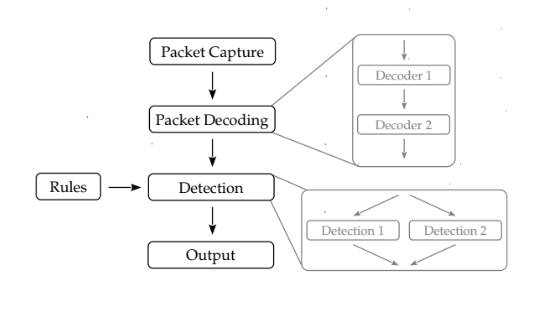
\includegraphics[width=90mm]{images/suricata-structure.png}
    \caption{Funzionamento del pattern matching}
    \label{}
  \end{center}
\end{figure}
Ogni pacchetto passante sull'interfaccia di rete monitorata dall'IDS viene quindi
decodificato e poi analizzato parallelamente per riscontrare similitudini con pi\`u pattern (rules).
Una tipica regola per il suddetto patter matching \`e nella forma seguente:
\begin{verbatim}
  alert tcp 1.1.1.1 8909 -> 192.168.1.0/24 80
\end{verbatim}
Viene quindi indicata l'azione da intraprendere (in questo caso 'alert'), il protocollo
, indirizzo/i di sorgente, porta/e sorgente, indirizzo/i di destinazione e porta/e di destinazione
del pacchetto con cui fare match.
Queste regole possono essere personalizzate oppure \`e possibile scaricarne di gi\`a confezionate
da molteplici siti che offrono questo servizio.
La praticit\`a dell'utilizzare questa specifica sintassi sta nel fatto che essa \`e quasi del
tutto identica a quella di Snort. Per cui le regole per l'uno o per l'altro software sono
intercambiabili.

\subsubsection{Altre caratteristiche}

Infine una delle caratteristiche fondamentali di Suricata sta nel fatto che esso pu\`o funzionare in
due modi distinti:
\begin{itemize}
  \item In modalit\`a online: viene monitorata una interfaccia specifica in modalit\`a {\it promisqua},
  ossia tutti i pacchetti passanti per quella determinata interfaccia vengono decodificati e analizzati.
  \item In modalita offline: viene monitorato un file pcap contenente del traffico
  "registrato" in precedenza e che costituisce un punto di riferimento per l'analisi
  prestazionale delle regole o dell'istanza di Suricata da analizzare.
\end{itemize}

Concludiamo quindi elencando i motivi che hanno portato durante le fasi di sperimentazione
alla scelta di Suricata rispetto ad altri software:
\begin{itemize}
  \item Velocit\`a (Multi-threading)
  \item Capacit\`a di analizzare pcap in modalit\`a offline
  \item Open Source
  \item Possibili\`a di analizzare facilmente i log grazie al formato in json
  \item Il fatto che si tratti di un software "giovane", pensato fin da
  subito per rispondere alle attuali esigenze di monitoraggio
\end{itemize}

\newpage


\section{sFlow}

L' esplosione del traffico internet sta portando a larghezze di banda superiori
e una maggiore necessit\`a di reti ad alta velocit\`a. Per analizzare e ottimizzare
le reti \`e necessario un sistema di monitoraggio efficiente. \cite{S1}

sFlow \cite{K1} \`e una tecnologia sviluppata dalla InMon Corporation per monitorare il traffico all'interno
di grandi reti contenenti
switches e routers che utilizza il campionamento di pacchetti. In particolare, esso
definisce i meccanismi di campionamento implementati
in un \emph{sFlow Agent} e il formato dei dati campionati mandati da tale Agent.

Il monitoraggio si compone di due elementi fondamentali:
\begin{itemize}
  \item {\bf sFlow Agent}: ovvero un qualsiasi apparato in grado di campionare
  i pacchetti secondo le specifiche di sFlow e di inviarli ad un {\it Collector}.
  l'Agent \`e un componente molto versatile ed estremamente performante dell'architettura
  sFlow che pu\`o essere impersonato anche da uno switch o da un router, senza degradarne
  le prestazioni.
  Il campionamento e la raccolta dei dati del nodo viene fatta in hardware e non presenta
  overhead nemmeno su reti Gigabit.
  \item {\bf sFlow Collector}: ovvero una macchina in qualsiasi parte del mondo in grado di raccogliere
  i dati sFlow e di elaborarli.
\end{itemize}

L'architettura e le modalit\`a di campionamento usati in sFlow offrono numerosi vantaggi
tra cui quello di avere una visione di tutta la rete ({\it network-wide}) in tempo
reale. La visione {\it network-wide} \`e possibile poich\`e sempre pi\`u produttori
stanno equipaggiando i loro apparati di rete con un modulo sFlow; inoltre recentemente
\`e stato aggiunto il supporto a sFlow anche all'interno di {\it OpenVSwitch}, un
famoso software usato nel campo della {\it Software Designed Networking}.
 La visione in tempo reale invece \`e permessa dal fatto che i pacchetti campionati
 vengono mandati al collector non appena essi passano per
l'agent.
Un ulteriore punto a favore sta nel fatto che si tratta di un' architettura
estremamente scalabile che permette di posizionare gli agent in diversi punti della rete,
o anche in reti diverse, garantendo una visione totale della rete anche in contesti
{\it Multi-homed}.

\subsection{Il campionamento}

Il campionamento \`e la parte fondamentale del protocollo sFlow, ed \`e anche
il motivo per cui esso si distacca da altre tecnologie simili come NetFlow.

sFlow usa due modalit\`a operative:
\begin{itemize}
  \item {\bf Counter Sampling} : un campione dei contatori delle interfacce dell'apparato, che viene
  schedulato internamente dall' Agent su base temporale ({\it polling}).
  \item {\bf Packet Based Sampling}: il campionamento di uno ogni N pacchetti
  sulla base di un opportuno parametro N ({\it sampling rate}). Questo tipo di campionamento non
  permette risultati accurati al 100\% ma quantomeno permette di avere risultati
  di un'accuratezza accettabile e comunque parametrizzabile
\end{itemize}

Il pacchetto campionato viene esportato verso l'sFlow Collector tramite UDP \cite{B1}.
La mancanza di affidabilit\`a nel meccanismo di trasporto UDP non influisce in modo
significativo sulla precisione delle misurazioni ottenute dall' Agent sFlow, poich\'e se
i Counter Sampling vengono persi, al superamento dell' intervallo di polling
successivo verranno inviati nuovi valori. Se invece vengono persi i Packet Flow Sample, questo si riflette in
una leggera riduzione della frequenza di campionamento effettiva.  L' uso di UDP
inoltre riduce la quantit\`a di memoria necessaria per il buffer dei dati. UDP \`e pi\`u
robusto di un meccanismo di trasporto  affidabile (es. TCP) perch\`e sotto sovraccarico
l' unico effetto sulle prestazioni complessive del sistema \`e un leggero aumento
del ritardo di trasmissione e un maggior numero di pacchetti persi, nessuno dei
quali ha un effetto significativo sul sistema di monitoraggio.

\newpage

\subsubsection{Sflow Datagram}

\begin{figure}[t!]
  \begin{center}                          %centra nel mezzo della pagina
    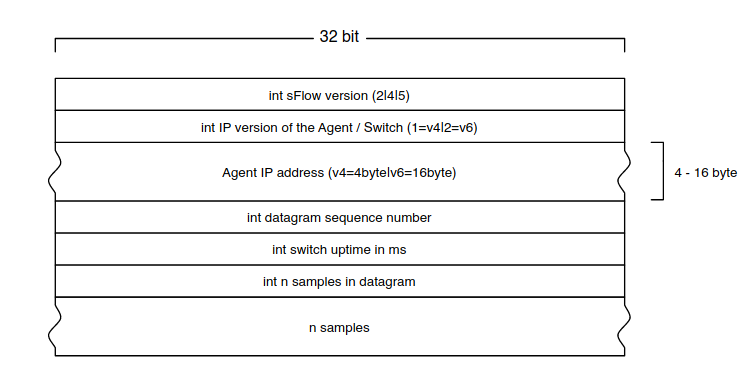
\includegraphics[width=90mm]{images/sflow-datagram.png}
    \caption{Datagram sFlow}
    \label{Datagram sFlow}
  \end{center}
\end{figure}

Il payload del pacchetto UDP inviato al Collector contiene l' sFlow Datagram, il quale
\`e composto da: versione di sFlow, ip dell'Agent, sequence-number, il numero di campioni
contenuti e fino a 10 campioni tra flow samples e counter samples (figura 1.2).

Un {\it flow sample} consiste di due parti:
\begin{itemize}
  \item un {\it packet data}: che contiene l'header del pacchetto campionato (il
  quale consiste nel pacchetto originale troncato fino ad una lunghezza parametrizzabile)
  \item un {\it extended data}: che contiene informazioni aggiuntive, ad esempio in
  caso di uno switch con VLANs abilitate fornisce la VLAN sorgente e di destinazione.
\end{itemize}

Come possiamo notare quindi avvengono due tipi di campionamento diversi: un campionamento
di un pacchetto ogni N e un troncamento del pacchetto designato fino ad una dimensione massima
T (solitamente fissata ad un massimo di 256 Bytes).
Occorre notare che il troncamento del pacchetto effettuato ci permette di avere
una visibili\`a dal Layer 2 al Layer 7 dello stack OSI \cite{B1}

E` necessario puntualizzare che il datagram contenente il {\it Packet Sample} a differenza del {\it Counter Sample}
viene inviato al collector appena il pacchetto viene campionato o comunque non oltre
un secondo pi\`u tardi dal campionamento, anche se non si \`e riempito il buffer di
10 campioni raccolti.

\subsection{Tools per l'utilizzo di sFlow}

La InMon Corporation mette a disposizione due tool fondamentali per l'utilizzo dello
standard sFlow, che svolgono i ruoli dell'Agent e del Collector.

\subsubsection{hostsflowd}
Hostsflowd \`e un tool per sistemi UNIX \footnote{Ne esiste una versione anche per Windows}
che svolge la funzione di Agent, ovvero osserva
i pacchetti passanti per una determinata interfaccia e applica ad essi i meccanismi di
campionamento discussi sopra. Esso permette di specificare tramite il suo file di configurazione:
la frequenza di campionamento ({\it Sampling Rate}), l'indirizzo del collector e la
sua porta, l'intervallo per il polling del {\it Counter Sample} e la grandezza dell'header
del pacchetto campionato.

Si tratta di un tool molto versatile e dai requisiti molto bassi, tuttavia durante
i test \`e emersa una limitazione importante, ossia che non \`e possibile
troncare pacchetti ad una dimensione pi\`u grande di 256 Byte, inoltre non \`e possibile
impostare un sampling rate di 1/1 (ovvero campionare tutto). Questo potrebbe non essere
una limitazione determinante in produzione ma in fase di testing si \`e stati costretti
a prendere strade alternative, che hanno portato allo sviluppo del simulatore {\it pcap2sflow}.
Ulteriori motivazioni di questa scelta saranno fornite nel capitolo 2.

\subsubsection{sflowtool}

Sflowtool \`e un toolkit per decodificare
dati sFlow. Esso svolge quindi la funzione di Collector, ed \`e in grado di stampare
in STDOUT i dati decodificati o, cosa molto pi\`u importante nel contesto di applicazione
di questa tesi, spacchettare i campioni e
riscriverli in formato pcap.

{\it Ad esempio con il comando seguente \`e possibile esportare i pacchetti campionati
in un file pcap che conterr\`a i campioni raccolti dall'Agent, troncati secondo i
parametri specificati nell'Agent:}
\begin{verbatim}
  sflowtool -t > capture.pcap
\end{verbatim}

\subsubsection{Alternative a sFlow}

Ci sono molte tecnologie che a prima vista potrebbero sembrare simili ad sFlow,
probabilmente per la presenza della parola "flow", tipo NetFlow, OpenFlow o IPFIX.
Tuttavia essi si differenziano da sFlow per alcuni motivi fondamentali:
NetFlow e IPFIX sono protocolli di esportazione del flusso che mirano ad aggregare i pacchetti in flussi.
Successivamente, i record di flusso vengono inviati a un punto di raccolta per la
conservazione e l' analisi. \cite{S1} sFlow, tuttavia, non ha alcuna nozione di flussi o
aggregazione di pacchetti.
Inoltre, mentre l' esportazione del flusso pu\`o essere eseguita con campionamento 1:1
(cio\`e considerando ogni pacchetto), questo non \`e tipicamente possibile con sFlow,
in quanto non \`e stato progettato per farlo. Il campionamento \`e parte integrante di
sFlow, con l' obiettivo di fornire scalabilit\`a per il monitoraggio in tutta la rete. \cite{S2}

La caratteristica fondamentale necessaria per la riuscita del progetto portato avanti in questa tesi
st\`a proprio nel fatto che i dati non siano dati aggregati, come avviene
in NetFlow o IPFIX. Un aggregazione dei dati non permette infatti un'analisi degli header
dei pacchetti invalidando quindi la funzionalit\`a di monitoraggio contro gli
attacchi informatici.

Come ulteriore prova si fornisce un esempio di dati provenienti da un sistema
di monitoraggio che utilizza NetFlow (con un ragionamento analogo \`e possibile
fornire la stessa prova per IPFIX).

Output del comando {\it nfdump}:
\begin{figure}[h!]
  \begin{center}                          %centra nel mezzo della pagina
    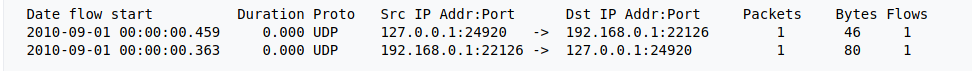
\includegraphics[width=\linewidth]{images/netflow.png}
    \caption{}
    \label{}
  \end{center}
\end{figure}

\newpage

\section{Packet sampling e Intrusion Detection}

La sicurezza delle reti, specie di quelle molto estese, \`e un problema tutt'oggi
presente e di un importanza vitale per qualsiasi azienda che operi nel settore ICT (Information and Communications Technologies).
Le minacce possono presentarsi in qualunque momento \cite{K3} e provenire sia dall'interno
che dall'esterno. Riuscire ad identificare queste minacce in tempo \`e il primo passo verso la soluzione di
questo difficile problema. Per fare ci\`o \`e necessario avere un'ampia e continua
sorveglianza della rete.
Storicamente la sorveglianza di una grande rete era (ed \`e tuttora) affidata a sonde ({\it probes}),
posizionate in punti strategici della rete. Questo \`e stato sufficientemente accurato
fino ad ora, ma visto l' aumento delle switched point to point network, il monitoraggio {\it probe-based} non
\`e pi\`u sufficiente.
Implementare il monitoraggio gi\`a dall'interno di uno switch o di router sta
diventando sempre pi\`u una necessit\`a. Tuttavia le esigenze di mercato tendono a preferire
l'ampiezza di banda sulla sicurezza, per cui la funzione di monitoraggio deve essere relegata come
funzione secondaria all'interno di questi apparati di rete. \`E necessario quindi che questa funzione
operi con il minimo overhead possibile, al fine di non degradare le prestazioni dell'apparato.
\`E qui che entra in gioco la tecnologia sFlow, essa permette di delegare la parte di analisi del traffico
ad un altro componente della rete ({\it il collector}), lasciando allo switch o al router le risorse per
effettuare le normali decisioni di smistamento dei pacchetti.

Il rilevamento delle intrusioni basato sui flow \`e un modo innovativo di rilevare
le intrusioni nelle reti ad alta velocit\`a. Il rilevamento delle intrusioni basato
sui flow controlla solo l' header del pacchetto e non ne analizza il {\it payload}.
Analizzare il {\it payload} del pacchetto infatti sarebbe computazionalmente inaccettabile
su reti di grandi dimensioni e con un elevato flusso di dati. Questa limitazione per\`o
nel caso di sFlow si presuppone che non invalidi la qualit\`a del sistema di monitoraggio
poich\`e la stragrande maggioranza degli attacchi \`e riconoscibile tramite un'analisi
degli header al di sopra del livello di Livello 3.

Vediamo ora pi\`u nel dettaglio come \`e possibile costruire con sFlow un sistema di monitoraggio efficace
e che rispetta le richieste di mercato:
\begin{itemize}
  \item Il sistema deve avere una sorveglianza continua network-wide: sFlow pu\`o essere configurato su ogni apparato di rete
  \item I dati devono essere sempre disponibili per rispondere efficacemente: sFlow manda immediatamente
  i pacchetti campionati al Collector con UDP
  \item I dati devono essere sufficientemente dettagliati per caratterizzare l'attacco: sFlow permette di
  esportare pi\`u di 128 Byte (comprendendo quindi ad esempio anche header di livello 7)
  \item Il sistema di monitoraggio non deve esporre gli apparato ad attacchi: sFlow non impatta sulle
  prestazioni degli apparati poich\`e viene effettuato in hardware inoltre il consumo di banda \`e limitato
  poich\`e i datagram sFlow sono ottimizzati
\end{itemize}

\subsection{Metodi di rilevazione flow-based}

L'analisi dei dati provenienti dai {\it flow generators} al fine di garantire una
rilevazione efficace della maggior parte degli attacchi ha portato nel corso degli anni
all'utilizzo di molteplici approcci, che utilizzano tre macroaree dell'intrusion
detection moderna:
\begin{itemize}
  \item {\it Statistical Analysis}
  \item {\it Machine Learning Analysis}
  \item {\it Signature-based Analysis}
\end{itemize}


I metodi statistici ({\it Statistical Analysis}) costruiscono un profilo del traffico
di rete normale utilizzando una funzione statistica dei parametri del traffico di rete;
questo profilo del traffico normale viene utilizzato per controllare il traffico in
arrivo al momento attuale; la somiglianza tra il traffico di rete e il profilo del
traffico di rete normale viene calcolata utilizzando appunto metodi statistici. Se la misura
di somiglianza \`e al di sopra della soglia predefinita, il flusso \`e marcato come
dannoso, altrimenti come flusso normale. \cite{S4} I metodi statistici non necessitano di conoscenza pregressa
di un determinato attacco per determinare se un campione contiene effettivamente un attacco, e questo si
\`e dimostrato particolarmente efficace nel rilevare attacchi di tipo DoS ({\it Denaial of
Service}). Essi tuttavia possono essere aggirati mantenendo l'impatto dell'attacco al di
sotto della soglia predefinita. Inoltre l'efficacia di questi metodi in reti reali
\`e minata dalla difficolt\`a intrinseca che sta nel calcolare le statistiche sul traffico.

I metodi che utilizzano tecniche di {\it Machine Learning} si basano principalmente,
su reti neurali, {\it Support Vector Matrix } (SVM), {\it Decision Tree} e {\it Clustering}.
Essi presentano numerosi vantaggi rispetto ai metodi statistici quali l'adattamento
del comportamento in base ad una finestra temporale. Inoltre i risultati degli esperimenti
condotti con Machine Learning hanno evidenziato un'ottimo tasso di riconoscimento degli
attacchi in un processo di "apprendimento" relativamente breve. Tuttavia anche questo metodo
ha degli svantaggi importanti come la difficolt\`a di generare dati campioni per
l'apprendimento, inoltre quest'ultimo si \`e rivelato computazionalmente molto costoso.
Infine essi hanno un alto tasso di falsi positivi (ovvero allarmi che vengono generati da un pacchetto che inveve era
benevolo).

In ultimo abbiamo la {\it Signature-based Analysis}, tema principale di questo elaborato,
che utilizza l'header dei pacchetti campionati per fare pattern matching con un dataset
di regole statiche. Questo approccio porta con se tutti i vantaggi e gli svantaggi
degli IDS Signature-based discussi nei paragrafi precedenti, con il solo svantaggio aggiunto di
non poter ricorrere all'utilizzo della Stateful Analysis poich\`e il campionamento
non garantisce che tutti i pacchetti di una determinata sessione siano catturati.
Inoltre occorre ribadire che tale metodo \`e utilizzabile solo nel caso in cui si abbiano a disposizione
almeno gli header di Livello 3, per quanto detto nella sezione "Alternative a sFlow",
da cui ci si accorge che sFlow rappresenta l'unica alternativa di applicazione.


\newpage

\section{Elasticsearch e lo stack ELK}

L'analisi dei dati, specie se di grosse dimensioni, come i dati generati dai test o
dai log, \`e un problema che va affrontato con sistematicit\`a al fine di poter
trarre delle conclusioni descrittive sul lavoro svolto. \`E stato necessario quindi
utilizzare tool appositamente studiati per la {\it Data Analysys} come lo stack ELK, ed
in particolare Kibana.

Elasticsearch \cite{E1} \`e un motore di ricerca basato su Lucene.
\`E un software con capacit\`a di ricerca full-text, multitenant e distribuito.
Possiede un' interfaccia web HTTP e una strutura schema-free di documenti con la sitassi JSON.
A differenza di un {\it Database Management System} relazionale, esso \`e {\it schema-free}
anche se non {\it schema-less} (come MongoDB per esempio) il che significa che non \`e
necessario definire i tipi (string, integer, ecc.) dei dati prima di inserirli,
ma comunque possibile. \cite{E4}
Elasticsearch \`e sviluppato in Java ed \`e rilasciato con licenza Open Source Apache.
I client ufficiali sono disponibili in Java,. NET (C#), PHP, Python, Apache Groovy e molti altri
linguaggi.
Secondo DB-Engines, \cite{E2} Elasticsearch \`e il motore di ricerca pi\`u popolare in ambito enterprise e
rappresenta un tool fondamentale nell'analisi e nella centralizzazione dei log.

Elasticsearch infatti \`e sviluppato, dallo stesso team, di pari passo con Logstash
e Kibana e i tre programmi insieme formano quello che viene chiamato lo stack ELK.

Esso si compone di tre componenti fondamentali:
\begin{itemize}
  \item {\bf Logstash} : \`e una "pipeline di elaborazione dati" che pu\`o raccogliere
  dati da varie fonti, trasformarli e inviarli a vari consumatori, tra cui Elasticsearch
  \item {\bf Elasticsearch} : come descritto prima, un database No-SQL particolarmente ottimizzato per la
  ricerca
  \item {\bf Kibana} : \`e uno strumento di visualizzazione web-based che si integra
  con Elasticsearch atto a fornire un modo efficace per navigare e visualizzare i dati,
  utilizzando una variet\`a di grafici, grafici e tabelle.
\end{itemize}


Lo stack ELK \`e ad oggi lo standard {\it de facto} per l'esplorazione dei log,
esso si va ad affiancare a tutti i programmi critici all'interno di una infrastruttura
e risulta particolarmente utile nell'esplorazione dei log degli IDS. Collegato ai log di
un IDS permette infatti
acquisire in pochissimi secondi conoscenza su cosa accade nella rete e su che tipo di attacchi
sono in corso. I dati vengono fruiti all'operatore in maniera veloce e comprensibile tramite
dashboard, fornendo una fotografia estremamente informativa dello stato attuale.

In figura \`e illustrato il funzionamento della pipeline di analisi usando lo stack
ELK.

\begin{figure}
  \begin{center}                          %centra nel mezzo della pagina
    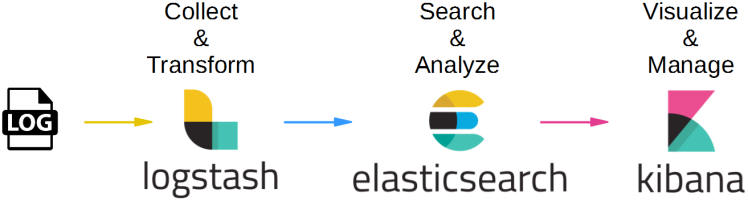
\includegraphics[width=90mm]{images/ELK-stack.png}
    \caption{Lo stack ELK}
    \label{}
  \end{center}
\end{figure}


\newpage

\chapter{Proposta}                %crea il capitolo
%%%%%%%%%%%%%%%%%%%%%%%%%%%%%%%%%%%%%%%%%imposta l'intestazione di pagina
\lhead[\fancyplain{}{\bfseries\thepage}]{\fancyplain{}{\bfseries\rightmark}}


In questo capitolo si va ad illustrare nel dettaglio quella che \`e stata ritenuta una possibile
proposta di soluzione al problema del monitoraggio basato su packet sampling. Si andranno
a descrivere i vari contesti di sperimentazione, i tool utilizzati e le modalit\`a di
utilizzo di questi ultimi. Si andr\`a poi ad introdurre il software {\it pcap2sflow}, sviluppato per
simulare il comportamento di sFlow e garantire una riproducibilit\`a dei test effettuati.
Infine si descriveranno le modalit\`a di analisi dei dati raccolti.

\section{sFlow + Suricata}

Data la natura del protocollo sFlow, ovvero quella di poter esportare l'header di
un numero parametrizzabile di pacchetti passanti attraverso un interfaccia di rete verso
un altro componente della rete, la conclusione pi\`u immediata a cui si \`e giunti
e stata quella di analizzare questi header campionati con l'IDS Suricata.
Come visto nel capitolo precedente, Suricata permette identificare possibili {\it threat}
tramite l'utilizzo di {\it rules}. La particolarit\`a di questo metodo sta nel fatto che
molte delle signature descritte all'interno delle rules, fanno riferimento proprio all'heder del
pacchetto. Questo rende Suricata un ottimo candidato per l'analisi di questi dati.

Come illustrato nel capitolo precedente, InMon Corp. mette gi\`a a disposizione dei
tool per realizzare questo tipo di architettura, ovvero {\bf hostsflowd} e {\bf sflowtools}.
Andiamo quindi ad illustrare quello che \`e stato il primo approccio verso l'analisi di
questa soluzione.

\subsection{L'architettura}

L'idea \`e quella di collocare un solo collector in un punto strategico di una rete e
inoltrare il traffico passante per tale collector verso un altro host su cui \`e installato
l'Agent e Suricata.

L'intera sperimentazione si basa su due macchine virtuali identiche chiamate {\it Generator} e {\it Collector}
con le caratteristiche elencate in tabella.

\begin{center}
  \begin{tabular}{| l | r |}
    \hline
    Numero di CPU & 2 \\ \hline
    Architettura del processore & x86\_64 \\ \hline
    RAM & 3GB \\ \hline
    Numero delle interfacce di rete & 2 \\ \hline
    Sistema operativo & Linux \\ \hline
    Distribuzione & Debian 8 \\ \hline
    Versione del Kernel & 4.9.0-4-amd64 \\ \hline
  \end{tabular}
\end{center}

\subsubsection{Installazione e configurazione}

Una volta create le macchine virtuali usando il programma VirtualBox \cite{EXP1} e vi \`e stato
installato Debian 8 \footnote{Si tralasciano i dettagli sulla creazione delle macchine e sull'installazione
di Debian, ma \`e comunque presente in bibliografia un riferimento rigurardo alla procedura seguita \cite{EXP10} \cite{EXP11} }.

Si \`e passato poi alla configurazione delle interfacce di rete, su entrambe le macchine, tramite il file \linebreak
{\verb /etc/network/interfaces }  come segue:

\paragraph{Generator}
\begin{verbatim}
# The primary network interface che comunica con il Collector
allow-hotplug enp0s3
iface enp0s3 inet dhcp

#Interfaccia di servizio
auto enp0s8
iface enp0s8 inet static
address 10.0.1.2
netmask 255.255.255.0

#interfaccia visibile dall'esterno per utilizzo con SSH
auto enp0s9
iface enp0s9 inet static
address 192.168.56.2
netmask 255.255.255.0

\end{verbatim}
\paragraph{Collector}
\begin{verbatim}
# The primary network interface che comunica con il Generator
allow-hotplug enp0s3
iface enp0s3 inet dhcp

#Interfaccia di servizio (non utilizzata)
auto enp0s8
iface enp0s8 inet static
address 10.0.1.3
netmask 255.255.255.0

#interfaccia visibile dall'esterno per utilizzo con SSH
auto enp0s9
iface enp0s9 inet static
address 192.168.56.3
netmask 255.255.255.0

\end{verbatim}

La topologia della rete aveva quindi una struttura uguale a quella rappresentata
in figura 2.1.

\begin{figure}
  \begin{center}                          %centra nel mezzo della pagina
    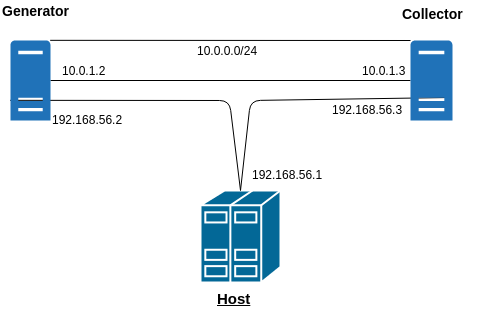
\includegraphics[width=90mm]{images/rete.png}
    \caption{Topologia della rete}
    \label{}
  \end{center}
\end{figure}

Si sono quindi installati i due programmi hostsflow e sflowtools su Collector e su
Generator rispettivamente.
Poi si \`e installato Suricata su Collector e si sono scaricate le regole base dal
sito di {\it Emerging Threats}. Inoltre si sono abilitati i log nel formato json. \cite{EXP2}
Per concludere si \`e proceduto all'installazione dello stack ELK per l'analisi dei log.

L'architettura finale del setup creato per le sperimentazioni aveva la struttura
mostrata in figura 2.2 .

\begin{figure}
  \begin{center}                          %centra nel mezzo della pagina
    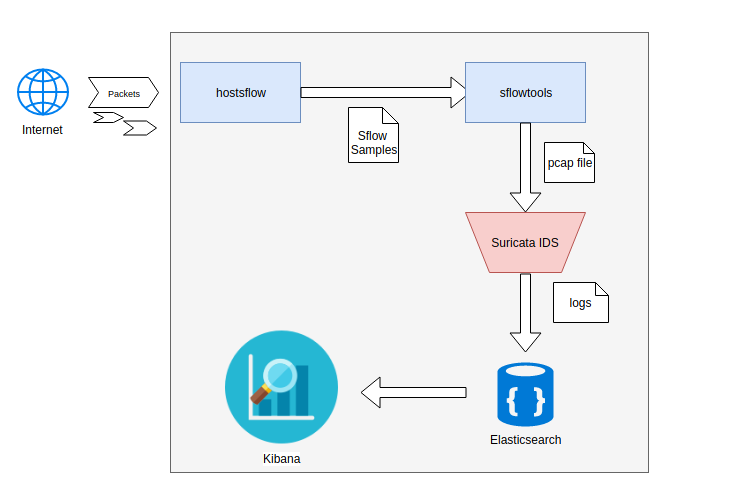
\includegraphics[width=90mm]{images/arch.png}
    \caption{Architettura I}
    \label{}
  \end{center}
\end{figure}

Si ha quindi che, hostsflow monitora l'interfaccia di rete {\verb enp0s8 } e invia i campioni incapsulati in
datagrams sFlow a sflowtools sulla porta standard 6343, quest'ultimo spacchetta i campioni e
li riscrive. Successivamente i pacchetti trascritti
da sflowtool vengono dati da analizzare a Suricata, il quale opera una {\it offline analysis}.
Infine i log generati da Suricata vengono trascritti all'interno di Elasticsearch utilizzando
lo script {\it elasticsearch\_feeder.py}. Ora che i dati sono indicizzati in Elasticsearch \`e
possibile esplorarli e creare delle visualizzazioni all'interno dell'interfaccia web di Kibana.

\section{Datasets}

Al fine di garantire la riproducibilit\`a dei risultati ottenuti da questo studio,
si \`e scelto di utilizzare una collezione di datasets spesso utilizzati nella letteratura
per il testing degli Intrusion Detection Systems \cite{EXP3}.

I dataset scelti per il testing sono stati:
\begin{itemize}
  \item DARPA Intrusion Detection Data Set (1999) \cite{EXP4}
  \item CTU-13 Dataset \cite{EXP5}
  \item ICtF 2010 {\it (International Capture the Flag, ed. 2010)} \cite{EXP6}
\end{itemize}

Il {\it DARPA Intrusion Detection Data Set (1999)} \`e un dataset composto da traffico misto,
 acquisito in tre settimane di training di un IDS. Nella prima e la terza settimana non
sono presenti attacchi mentre nella seconda settimana sono stati eseguiti degli attacchi
principalmente mirati a far scattare le regole degli IDS oggetto di test.

Il {\it CTU-13} \`e un dataset sul traffico {\it botnet} che \`e stato acquisito nell' Universit\'a CTU,
Repubblica Ceca, nel 2011. L' obiettivo del dataset era quello di ottenere un' ampia cattura
del traffico delle botnet reali mescolato al traffico normale e al traffico di sottofondo.
Il set di dati CTU-13 consiste in tredici acquisizioni (chiamate scenari) di diversi campioni
di botnet. In ogni scenario \`e stato eseguito un malware specifico, che ha utilizzato
diversi protocolli e ha eseguito diverse azioni

Infine {\it ICtF 2010} \`e un dataset ricavato dal traffico generato durante l'edizione del
2010 dell'International Capture the Flag di Santa Barbara. Si tratta quindi di un dataset
derivante da una competizione in cui si mettono alla prova le capacit\`a di {\it penetration
testing} dei partecipanti. Esso costituisce per questo motivo un ottimo dataset di testing poich\`e
, a differenza dei precedenti, non \`e stato
costruito appositamente per studiare determinati comportamenti di un IDS in specifiche
condizioni.

\section{Metodologie di test}

Si vanno adesso ad elencare le metodologie dei test effettuati, la terminologia, l'organizzazione delle
directory e lo schema del database di Elasticsearch.

\subsection{Terminologia}

\begin{itemize}
  \item {\it \bf Sampling Rate} : \`e la frequenza di campionamento operata dall'Agent sFlow,
  ad esempio un Sampling Rate uguale a 4 vuol dire che ogni 4 pacchetti uno viene
  campionato
  \item {\it \bf Troncamento} : \`e la dimensione massima del pacchetto scelto per il campionamento
  , tale pacchetto viene troncato fino a {\it t} Bytes e inviato al collector.
  \item {\it \bf Setup On-Wire} : \`e il setup per cui il traffico viene inoltrato interamente
  a Suricata per l'analisi. Esso corrisponde al normale utilizzo del software in questione.
  \item {\it \bf Alert} : \`e un messaggio di allarme dell' IDS che notifica l'amministratore
  di una violazione delle policy di sicurezza.
\end{itemize}


L'obbiettivo dei test effettuati  \`e verificare se gli alert sollevati da Suricata
in modalit\`a On-Wire sono paragonabili a quelli che si ottengono fornendo ad esso solo
i dati parziali derivanti da sFlow.
Inoltre si vuole verificare l'incisivit\`a dei parametri di sampling rate e troncamento e
se essi siano indipendenti l'uno dall'altro.

\subsection{Struttura delle directory}

Con l'obiettivo di tenere organizzati i risultati dei numerosi test effettuati si
\`e scelto di seguire una rigorosa struttura delle directory e dei file.

Partendo dalla directory {\it root} del progetto si trovano le sottodirectory
dei dataset analizzati, all'interno di esse vi sono i test numerati da 1 a {\it n} e all'interno
di ogni directory di test troviamo i files: {\verb alert-debug.log }, {\verb eve.json },
{\verb fast.log }, {\verb pcap_size.txt }, {\verb stats.log }, {\verb test_info.txt }. Dove:
\begin{itemize}
  \item {\verb alert-debug.log }, {\verb eve.json }, {\verb fast.log }, {\verb stats.log }
  rappresentano i log di Suricata relativi al test in esame
  \item {\verb pcap_size.txt }, {\verb test_info.txt } rappresentano rispettivamente la quantit\`a di
  traffico generato dal tipo di campionamento scelto e i parametri di campionamento.
\end{itemize}
\begin{verbatim}
  /root
    /dataset-name
      /number of test
        alert.debug
        eve.json
        fast.log
        pcap_size.txt
        stats.log
        test_ingo.txt
\end{verbatim}

\subsection{Il cuore degli esperimenti}

Inizialmente, soprattutto nelle prime fasi di analisi di fattibilit\`a dell'applicazione oggetto
di studio i test sono stati effettuati a mano, utilizando come solo supporto una checklist, che
assicurava la coerenza della struttura delle directory cos\`i come del contenuto dei
risultati dei test stessi.

Sulla macchina Generator \`e stato configurato hostsflowd tramite il suo file di
configurazione {\verb /etc/hsflowd.conf } includendo i seguenti campi:
\begin{verbatim}
  # hsflowd configuration file
  # http://sflow.net/host-sflow-linux-config.php

sflow {
     agent = enp0s8
     polling = 30
     sampling = 2
     collector { ip=10.0.0.3 udpport=6343 }
     pcap { dev =  enp0s8 }
     headerBytes = 128
}
\end{verbatim}

e si avvia hsflowd con il comando :
\begin{verbatim}
  hsflowd -d
\end{verbatim}

In questo modo l'Agent hsflowd analizza il traffico passante per l'interfaccia di
rete enp0s8 e invia i datagram sFlow alla macchina Collector, sul quale \`e in esecuzione
il programma sflowtool
\begin{verbatim}
sflowtool -p 6343 -t | suricata -c /etc/suricata/suricata.yaml -r -

\end{verbatim}

Nella seconda parte del comando di sopra, il traffico viene passato a Suricata
che effettua un analisi offline trattando l'input come se fosse un normale file pcap.

A questo punto tutto \`e pronto e il traffico dei dataset pu\`o essere iniettato
nella rete all'interfaccia monitorata da hsflowd. Quindi, posizionandosi sul Generator stesso si esegue il
comando:
\begin{verbatim}
  tcpreplay -i enp0s8 <file pcap da analizzare>
\end{verbatim}

\paragraph{Problemi}

\`E tuttavia emerso un problema da questa metodologia, tcpreplay cerca di iniettare
il traffico nell'interfaccia rispettando, come e giusto che sia, il timing di arrivo
dei pacchetti registrati nel file pcap. Questo sebbene assicuri una precisione certamente
desiderabile oltre a garantire la riproducibilit\`a dei test, non \`e una strada percorribile
(almeno per gli obiettivi di questa tesi) poich\`e i test richiederebbero troppo tempo per
essere portati a termine.
\`E altres\'i vero che \`e possibile istruire tcpreplay di non rispettare il timing,
ma questo andrebbe a invalidare quei regole di Suricata che fanno affidamento su di esso,
come ad esempio il rilevamento del famoso attacco {\it Slow HTTP}.

Inoltre, riguardo al voler determinare la l'incisivit\`a dei parametri sampling rate e
troncamento, \`e emerso che il programma utilizzato come Agent, hsflowd, non \`e sufficientemente
parametrizzabile.
In particolare la dimensione massima del
pacchetto che pu\`o essere esportato, ovvero quello che viene chiamto {\it header size} e che abbiamo
identificato come troncamento, \`e {\it hard-coded} ad un massimo di 256 Bytes.
Sebbene sia stato spiegato dalla InMon Corp. che tale dimensione massima \`e dovuta all'architettura
di sFlow e che \`e necessaria per garantire una scalabilit\`a del prodotto, alle
finalit\`a di testing questa si \`e rivelata una grossa limitazione, soprattuto quando i
risultati ottenuti si sono posti in contraddizione con quanto ci si aspettava.

In definitiva, sebbene questo primo approccio \`e stato determinante per verificare
la fattibilit\`a di affiancare sFlow a Suricata esso non \`e per nulla soddisfacente
ai fini della valutazione di efficienza.



\section{Una soluzione di testing alternativa}


Per quanto descritto nella sezione precedente, si \`e resa necessaria
una nuova modalit\`a di test, che sia meno dipendente dall'implementazione
di tutta la tecnologia \`e che lasci sufficienti margini di sperimentazione,
anche se questo vuol dire uscire dai paradigmi della tecnologia sFlow.


\subsection{Pcap2sFlow}

Si \`e sviluppato quindi un emulatore di sFlow che converte un file pcap in input,
in un altro file pcap contenente pacchetti campionati ricalcando le tecniche sFlow.

Si tratta di un programma scritto in C che utilizza la {\it libpcap } \cite{EXP7},
una libreria C per analizzare il traffico {\it live} o {\it captured}.

In particolare si sono utilizzate le seguenti funzioni di libreria:
\begin{verbatim}
pcap_dumper_t *pcap_dump_open(pcap_t *p, const char *fname);
\end{verbatim}

che apre il livecapture o il file pcap da cui leggere i pacchetti,

\begin{verbatim}
int pcap_loop(pcap_t *p, int cnt, pcap_handler callback, u_char *user);
\end{verbatim}

che processa i pacchetti da un livecapture o, come nel nostro caso da un {\it "savefile"},
ovvero un file in formato pcap, e ovviamente infine

\begin{verbatim}
void pcap_close(pcap_t *p);
\end{verbatim}

per chiudere il "savefile".

\subsubsection{Meccanismi di campionamento}

Per emulare il comportamento di sFlow occorre applicare lo stesso metodo di campionamento
utilizzato da quest'ultimo per scegliere quale pacchetto campionare e come troncare il
pacchetto in questione.

Si \`e scelto di prendere in considerazione solo il {\it Packet Sample} e di
tralasciare il {\it Counter Sample} poich\`e quest'ultimo non gioca alcun ruolo nel
IDS studiato (si veda la sezione 1.2.1).

Il Pachet Sampling all'interno di sFlow utilizza un meccanismo di randomizzazione
per determinare il pacchetto designato al campionamento. Pcap2sFlow allo stesso modo
divide il file da campionare in {\it windows} (finestre) della dimensione del parametro
{\it sampling rate}. All'interno di ogni finestra esso sceglie in modo random il pacchetto
da campionare. Di seguito sono riportati i listati dell'implementazione di tali
funzioni.

\begin{verbatim}
void select_random (cap_stat *stat) {
  //seleziona il prossimo pacchetto in modo random partendo
  //dall'ultima finestra considerata
  srand ( time(NULL) ) ;
  int x = rand();
  stat->s = stat->start + ( x % stat->n ) ;
}
void next_window (cap_stat *stat){
    //analizza la successiva finestra di pacchetti
    stat->start = stat->stop + 1;
    stat->stop = stat->stop + 1 + stat->n;
    select_random(stat);
}

bool to_sample ( cap_stat *sampler_info ) {
    //se n == 1 allora disattiva il campionamento e salva tutti
    //i pacchetti
    if (sampler_info->n == 1) return true;

    //controlla se il pacchetto corrente deve essere campionato
    if (sampler_info->curr_sample < sampler_info->start) {
        //se sono andato avanti con la window ma il cursore e`
        //ancora indietro questo pacchetto sara` sicuramente
        //da scartare
        sampler_info->curr_sample++;
        return false;
    }
    if (sampler_info->curr_sample == sampler_info->s) {
        //se il pacchetto corrente e` quello designato per essere
        //campionato avanza e rispondi true
        sampler_info->curr_sample++;
        next_window(sampler_info);
        return true;
    }
    else {
        sampler_info->curr_sample++;
        return false;
    }
}
\end{verbatim}

Nel testo dell'RFC 3176 viene detto che il seed della funzione {\verb select_random } non
dovrebbe essere alimentato con il tempo, come invece \`e stato fatto in pcap2sflow, poich\`e esso potrebbe non essere abbastanza
casuale in reti con un elevato {\it throughput}. Infatti in quel contesto la velocit\`a di aggiornamento delle windows
potrebbe essere pi\`u veloce della velocit\`a di aggiornamento del tempo. Tuttavia si \`e
ritenuto che nel contesto applicativo dell'esperimento questo non possa accadere.

Infine occorre troncare il pacchetto secondo una dimensione parametrizzabile,
e questo viene effettuato dalla seguente funzione:

\begin{verbatim}
void save_packet (cap_stat *s, const struct pcap_pkthdr *header,
                  const u_char *packet){
    if (s->truncate_b == 0) {
        //0 viene considerato come valore di default per
        //"salva tutto il pacchetto"
        pcap_dump((u_char *)s->pdumper, header, packet);
        return;
    }
    if (header->caplen > s->truncate_b) {
        u_char *new_packet = malloc(s->truncate_b);
        memcpy(new_packet,packet,s->truncate_b);
        pcap_dump((u_char *)s->pdumper, header, new_packet);
        free(new_packet);
    }
    else {
        pcap_dump((u_char *)s->pdumper, header, packet); } }
\end{verbatim}

Si \`e inoltre utilizzata la funzione di libreria {\it getopt} per rendere
il programma altamente parametrizzabile e {\it "script-friendly"}.
Con il parametro {\verb --help } \`e possibile visualizzare tutte le opzioni disponibili:

\begin{verbatim}

root@collector:# ./pcap2sflow --help
usage: ./pcap2sflow --infile <input_file.pcap> --outfile
        <output_file.pcap>

options:
-t      --trunkate-pkts <bytes>    truncate packet size to (bytes)
                                   size
-n      --no-truncate-pkts         do not truncate packets
-s      --sample-n <N>             sample 1 every N packets seen
-N      --no-sample                do not sample every N packets,
                                   take them all!
-h      --help                     show this help

\end{verbatim}

\section{Metodologia di test 2}

Data l'enormit\`a dei dataset da testare ed il numero di parametri che si intendevano
testare, il lavoro di testing e catalogazione \`e stato interamente svolto mediante l'uso di
script in Bash e Python. Quando ci si \`e chiesti se sviluppare un programma unico
per il test o una {\it suite} di tools si \`e scelto di abbracciare la filosofia Linux
del {\it "Do One Thing And Do It Well"} \cite{EXP12}, infatti un programma unico, date le
molte sfaccettature del progetto, sarebbe stato poco pratico.

Solitamente (tranne nel caso del dataset di DARPA) il {\it dump} del traffico era
diviso in segmenti della dimensione di 400 Megabyte circa. Lo script sviluppato si
occupa quindi di prendere ogni singolo file, campionarlo con pcap2sflow e far analizzare
a Suricata il file cos\`i generato. Infine si occupa di salvarne i risultati, ovvero i log e la
dimensione del file pcap dopo il campionamento.

In questo modo \`e stato possibile semplificare l'architettura illustrata precedentemente
in figura 2.2 con quella della figura 2.3, in cui si pu\`o notare che il software
pcap2sflow ha sostituito sia hostsflow che sflowtools, impersonando quindi sia
l'Agent che il Collector.

\begin{figure}
  \begin{center}                          %centra nel mezzo della pagina
    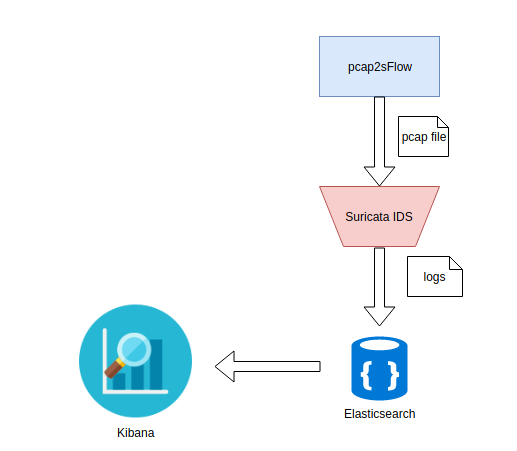
\includegraphics[width=90mm]{images/arch-2.png}
    \caption{Architettura II}
    \label{}
  \end{center}
\end{figure}

Si \`e prestata particolare attenzione durante le fasi di test alle performance e
al tempo di generazione dei risultati. Ad esempio, sebbene si possa campionare un file
pcap e subito darlo ad analizzare a Suricata, con il comando:
\begin{verbatim}
./pcap2sflow -i <pcap file> -s 100 -t 128 -o - | \
      suricata -c /etc/suricata/suricata.yaml -r -
\end{verbatim}
per ogni test che si sarebbe andato ad effettuare Suricata avrebbe dovuto ricaricare
tutto il core e tutte le regole. Questo si traduceva in uno spreco considerevole di tempo
che avrebbe allungato il tempo di esecuzione dei test. Allora si \`e optato per una
soluzione pi\`u moderna della classica PIPE di Linux che utilizza l'interfaccia
a {\it socket unix} di Suricata. Tramite questa interfaccia \`e possibile caricare una
volta sola il core e le regole e aggiungere in una coda i file pcap da analizzare.
Si \`e utilizzato per questo motivo il comando
\begin{verbatim}
suricatasc --command "pcap-file <file_pcap> <directory di log>"
\end{verbatim}

\section{Analisi dei risultati con Kibana e Elasticsearch}

Passiamo adesso alla descrizione di come i log e i dati in generale derivati dai
test effettuati siano stati organizzati per fornirne una rappresentazione informativa.
Si \`e utilizzato, come anticipato in precedenza Kibana ed Elasticsearch, ma non si
\`e utilizzato come avviene di solito, il terzo componente dello stack, ovvero Logstash.
Questo perch\`e la tipologia di dati raccolti necessitava di una manipolazione pi\`u approfondita di
quella che poteva fornirci Logstash. \`E stato necessario infatti scrivere un piccolo programma
Python, {\it elasticsearch\_feeder }, che attraversa tutte le directory dei risultati dei test e arricchisce i dati degli
alert con quelli dei parametri di campionamento e troncamento.

Un tipico alert di Suricata che \`e possibile trovare dentro il file eve.json \`e il
seguente:
\begin{verbatim}
{"timestamp":"1999-03-08T15:48:07.793208-0600","flow_id":3806400292,
"pcap_cnt":516386,"event_type":"alert","src_ip":"172.16.112.149",
"src_port":23, "dest_ip":"135.13.216.191","dest_port":20945,
"proto":"TCP",
  "alert":{"action":"allowed","gid":1,"signature_id":2019284,"rev":3,
  "signature":"ET ATTACK_RESPONSE Output of id command from HTTP server",
  "category":"Potentially Bad Traffic","severity":2}}
\end{verbatim}

Ognuno di questi alert rappresenta all'interno del database Elasticsearch un
documento.
Per ogni dataset \`e stato definito lo schema dell'index di Elasticsearch, come
nell'esempio seguente sul dataset di ICtF2010:
\begin{verbatim}
  {
    "ictf2010": {
      "aliases": {},
      "mappings": {
        "alerts": {
          "properties": { "adaptive_sampling": { "type": "boolean" },
            "alert": {
              "properties": {
                "category": {
                  "type": "text",
                  "fields": {
                    "keyword": {
                      "type": "keyword",
                      "ignore_above": 256 } } },
                "signature": {
                  "type": "text",
                  "fields": {
                    "keyword": {
                      "type": "keyword",
                      "ignore_above": 256 } } } } },
            "category": {
              "type": "text",
              "fields": {
                "keyword": {
                  "type": "keyword",
                  "ignore_above": 256 } } },
            "dest_ip": {
              "type": "text",
              "fields": {
                "keyword": {
                  "type": "keyword",
                  "ignore_above": 256 } } },
            "dest_port": { "type": "long" },
            "filename": {
              "type": "text",
              "fields": {
                "keyword": {
                  "type": "keyword",
                  "ignore_above": 256 } } },
            "proto": {
              "type": "text",
              "fields": {
                "keyword": {
                  "type": "keyword",
                  "ignore_above": 256 } } },
            "sampling": { "type": "long" },
            "signature": {
              "type": "text",
              "fields": {
                "keyword": {
                  "type": "keyword",
                  "ignore_above": 256 } } },
            "src_ip": {
              "type": "text",
              "fields": {
                "keyword": {
                  "type": "keyword",
                  "ignore_above": 256 } } },
            "timestamp": {
              "type": "date",
              "format": "yyyy'-'MM'-'dd'T'HH':'mm':'ss'.'SSSSSSZ" },
            "traffic": { "type": "long" },
            "truncate": {
              "type": "long" } } } },
      "settings": {
        "index": {
          "refresh_interval": "10s",
          "number_of_shards": "5",
          "provided_name": "ictf2010",
          "number_of_replicas": "1", } } } }
\end{verbatim}

Una volta creato l'index si \`e passati alla popolazione del database con
il programma Python elasticsearch\_feeder.py
Vista la grande quantit\`a di log \footnote{Si sono raggiunti 12 GB di log solo per il
testing del dataset ICtF2010}, si \`e ottimizzato l'inserimento utilizzando la
funzione di Elasticsearch {\it bulk index}.

Si \`e allora disabilitato temporaneamente il refresh degli index \cite{EXP8} \cite{EXP9}
\begin{verbatim}
PUT /ictf2010/_settings
{
    "index" : {
        "refresh_interval" : "-1"
    }
}
\end{verbatim}

E alla fine di ogni bulk index il valore \`e stato ripristinato ed \`e stato forzato
il merging dei segmenti:
\begin{verbatim}
PUT /ictf2010/_settings
{
    "index" : {
        "refresh_interval" : "10s"
    }
}

POST /twitter/_forcemerge?max_num_segments=5
\end{verbatim}

PARLARE DELL'INVERTED INDEX e di come ha ridotto le quantit\`a dei log

\subsubsection{Analisi dei falsi positivi}

Di fondamentale importanza nell'analisi prestazionale di un IDS \`e il conteggio
dei falsi positivi, ovvero di quegli alert sollevati dall'IDS a partire da un traffico
che era invece benevolo.

La valutazione dei falsi positivi \`e stata effettuata mediante un altro programma
Python, scritto appositamente sempre utilizzando le API di Elasticsearch.
Non \`e stato possibile infatti conteggiare i falsi positivi gi\`a dall'interno di
Kibana a partire dai dati gi\`a presenti poich\`e Elasticsearch non permette, a
differenza dei database relazionali, di effettuare delle subqueries.

Il programma Python, che va sotto il nome di false\_positives.py, confronta le signature
rilevate con i vari parametri di sampling rate e troncamento testati con le signature
del setup On-Wire. Il numero di falsi positivi per ogni signature ricavati dalla sottrazione dei
due valori \`e stata aggiunta in un ulteriore index, appositamente creato per il conteggio
dei falsi positivi.

false\_positives.py effettua una query con aggregazione sul valore "signature.keyword" nei
documenti con sampling rate = 1 e truncate = 600 (presi come riferimento per il setup On-Wire)
ne salva i valori e poi per ogni combinazione
di parametri effettua una seconda query con aggregazione sullo stesso valore; infine la differenza
tra i due valori ottenuta viene usata per creare tanti documenti quanti sono i falsi positivi.
Occorre notare che sebbene si creino molti documenti, data la struttura di Elasticsearch
e del suo Inverted Index, questo non occupa molto spazio e se ne guadagna in comodit\`a una volta che
si proceder\`a col creare le visualizzazioni.



\chapter{Discussione dei risultati}                %crea il capitolo
%%%%%%%%%%%%%%%%%%%%%%%%%%%%%%%%%%%%%%%%%imposta l'intestazione di pagina
\lhead[\fancyplain{}{\bfseries\thepage}]{\fancyplain{}{\bfseries\rightmark}}

In questo capitolo si vanno ad elencare i criteri di valutazione dei risultati
ottenuti dai test e se ne illustreranno e discuteranno i contenuti degli stessi.

Infine si proporr\`a un approccio alternativo al campionamento statico, ovvero
il campionamento adattivo.

\section{Criteri di valutazione}
In ogni contesto di sperimentazione, ovvero al variare di parametri dei test e di
dataset si sono osservati i comportamenti dei seguenti indicatori:
\begin{itemize}
  \item {\bf Alert} : la quantit\`a totale di alert sollevati da suricata
  \item {\bf Falsi positivi} : la quantit\`a di alert che nel setup On-Wire
  non \`e stata rilevata, e che per questo motivo costituisce sicuramente un false positivo
  \item {\bf Signature} : la tipologia di signature rilevata e la loro quantit\`a
  \item {\bf Traffico}: la quantit\`a in Bytes di traffico inviata per l'analisi
  a Suricata
  \item{\bf Capacit\`a a posteriori di identificare la sorgente e la destinazione di un
  attacco} : Questo indicatore risulta particolarmente utile nel campo dell'analisi forense,
  ovvero consente di identificare una volta scoperto l'attacco quali sono stati gli
  host coinvolti e da dove provenivano gli attaccanti.
\end{itemize}







%%%%%%%%%%%%%%%%%%%%%%%%%%%%%%%%%%%%%%%%%non numera l'ultima pagina sinistra
\clearpage{\pagestyle{empty}\cleardoublepage}
%%%%%%%%%%%%%%%%%%%%%%%%%%%%%%%%%%%%%%%%%per fare le conclusioni
\chapter*{Conclusioni}
%%%%%%%%%%%%%%%%%%%%%%%%%%%%%%%%%%%%%%%%%imposta l'intestazione di pagina
\rhead[\fancyplain{}{\bfseries
CONCLUSIONI}]{\fancyplain{}{\bfseries\thepage}}
\lhead[\fancyplain{}{\bfseries\thepage}]{\fancyplain{}{\bfseries
CONCLUSIONI}}
%%%%%%%%%%%%%%%%%%%%%%%%%%%%%%%%%%%%%%%%%aggiunge la voce Conclusioni
                                        %   nell'indice
\addcontentsline{toc}{chapter}{Conclusioni}
%%%%%%%%%%%%%%%%%%%%%%%%%%%%%%%%%%%%%%%%%imposta l'intestazione di pagina
\renewcommand{\chaptermark}[1]{\markright{\thechapter \ #1}{}}
\lhead[\fancyplain{}{\bfseries\thepage}]{\fancyplain{}{\bfseries\rightmark}}
\appendix                               %imposta le appendici
\chapter{Prima Appendice}               %crea l'appendice
%%%%%%%%%%%%%%%%%%%%%%%%%%%%%%%%%%%%%%%%%imposta l'intestazione di pagina
\rhead[\fancyplain{}{\bfseries \thechapter \:Prima Appendice}]
{\fancyplain{}{\bfseries\thepage}}
\chapter{Seconda Appendice}             %crea l'appendice
%%%%%%%%%%%%%%%%%%%%%%%%%%%%%%%%%%%%%%%%%imposta l'intestazione di pagina
\rhead[\fancyplain{}{\bfseries \thechapter \:Seconda Appendice}]
{\fancyplain{}{\bfseries\thepage}}
\begin{thebibliography}{90}             %crea l'ambiente bibliografia
\rhead[\fancyplain{}{\bfseries \leftmark}]{\fancyplain{}{\bfseries
\thepage}}
%%%%%%%%%%%%%%%%%%%%%%%%%%%%%%%%%%%%%%%%%aggiunge la voce Bibliografia
                                        %   nell'indice
\addcontentsline{toc}{chapter}{Bibliografia}
%%%%%%%%%%%%%%%%%%%%%%%%%%%%%%%%%%%%%%%%%provare anche questo comando:
%%%%%%%%%%%\addcontentsline{toc}{chapter}{\numberline{}{Bibliografia}}
\bibitem{K1} RFC 3176 InMon Corporation's sFlow for monitoring traffic in Switched
and Routed Networks
\bibitem{K2} A survery on Network Security Monitoring System,
Ibrahim Ghafir, Vaclav Prenosil, Jakub Svoboda, Mohammad Hammoudeh,
 2016 4th International Conference on Future Internet of Things and Cloud Workshops
\bibitem{K3} Traffic Monitoring with Packet-Based Sampling for Defense against Security Threats, Joseph Reves ans Sonia Panchen
\bibitem{K4} "NIST – Guide to Intrusion Detection and Prevention Systems (IDPS)" (PDF). February 2007.
\bibitem{K5} https://ossec.github.io/
\bibitem{K6} https://github.com/OISF/suricata
\bibitem{K7} https://www.snort.org/
\bibitem{K8} https://www.bro.org
\bibitem{K9} https://www.ntop.org/products/packet-capture/pf\_ring/
\bibitem{S1} sFlow, I Can Feel Your Traffic, Elisa Jasinska, Amsterdam Internet Exchange


\bibitem{B1} Reti di Calcolatori, Larry Peterson, Bruce Davie, Apogeo, 2012

\bibitem{S1} Hofstede, Rick; Celeda, Pavel; Trammell, Brian; Drago, Idilio; Sadre, Ramin; Sperotto, Anna; Pras, Aiko. "Flow Monitoring Explained: From Packet Capture to Data Analysis with NetFlow and IPFIX". IEEE Communications Surveys & Tutorials. IEEE Communications Society
\bibitem{S2} http://blog.sflow.com/2009/05/scalability-and-accuracy-of-packet.html
\bibitem{S3} Flow-based intrusion detection: Techniquesand challenges, Muhammad Fahad Umer, Muhammad Sher, Yaxin Bi. Computers \& Security 70 (2017) 238-254
\bibitem{S4} Intrusion detection system: A comprehensive review, Hung-JenLiao, Chun-HungRichard Lin,Ying-ChihLin, Kuang-YuanTung

\bibitem{E1} https://www.elastic.co/
\bibitem{E2} https://db-engines.com/en/ranking/search+engine
\bibitem{E4} SCADA STATISTICS MONITORING USING THE Elastic Stack(Elasticsearch, Logstash, Kibana), James Hamilton, Brad Schofield, Manuel Gonzalez Berges, Jean-Charles TournierCERN, Geneva, Switzerland

\bibitem{EXP1} https://www.virtualbox.org/
\bibitem{EXP2} https://rules.emergingthreats.net/
\bibitem{EXP3} Quantitative Analysis of Intrusion Detection Systems: Snort and Suricata, Joshua S. White , Thomas T. Fitzsimmons , Jeanna N. Matthews
\bibitem{EXP4} https://www.ll.mit.edu/ideval/data/1999data.html
\bibitem{EXP5} https://mcfp.weebly.com/the-ctu-13-dataset-a-labeled-dataset-with-botnet-normal-and-background-traffic.html
\bibitem{EXP6} https://ictf.cs.ucsb.edu/pages/the-2010-ictf.html
\bibitem{EXP7} http://www.tcpdump.org/
\bibitem{EXP8} https://www.elastic.co/guide/en/elasticsearch/reference/current/tune-for-indexing-speed.html
\bibitem{EXP9} https://www.elastic.co/guide/en/elasticsearch/reference/current/indices-update-settings.html
\bibitem{EXP10} https://docs.oracle.com/cd/E26217_01/E26796/html/qs-create-vm.html
\bibitem{EXP11} https://www.debian.org/releases/jessie/amd64/
\bibitem{EXP12} Raymond, Eric S. (2003-09-23). "Basics of the Unix Philosophy". The Art of Unix Programming. Addison-Wesley Professional
\end{thebibliography}
%%%%%%%%%%%%%%%%%%%%%%%%%%%%%%%%%%%%%%%%%non numera l'ultima pagina sinistra
\clearpage{\pagestyle{empty}\cleardoublepage}
\chapter*{Ringraziamenti}
\thispagestyle{empty}
\end{document}
